	\chapter{Merging values through small cycles -mv}
	
	Let assume that we have two facts $u_i, u_j$ and two actions. Each action has only one effect and zero prevail precondition. One action has got effect of type $<u_i,u_j>$ and the second one has got opposite effect to this one. So, we have two facts and can get from one to another by applying one of these actions. This is possible because the actions do not have any other side effect nor precondition. 
	
	The reduction works in the way that the two facts are merged to one. Such a reduction is very practical because it can reduce number of facts and also another reduction may arise.
	
	\begin{figure}
		\begin{subfigure}[b]{0.4\textwidth}
			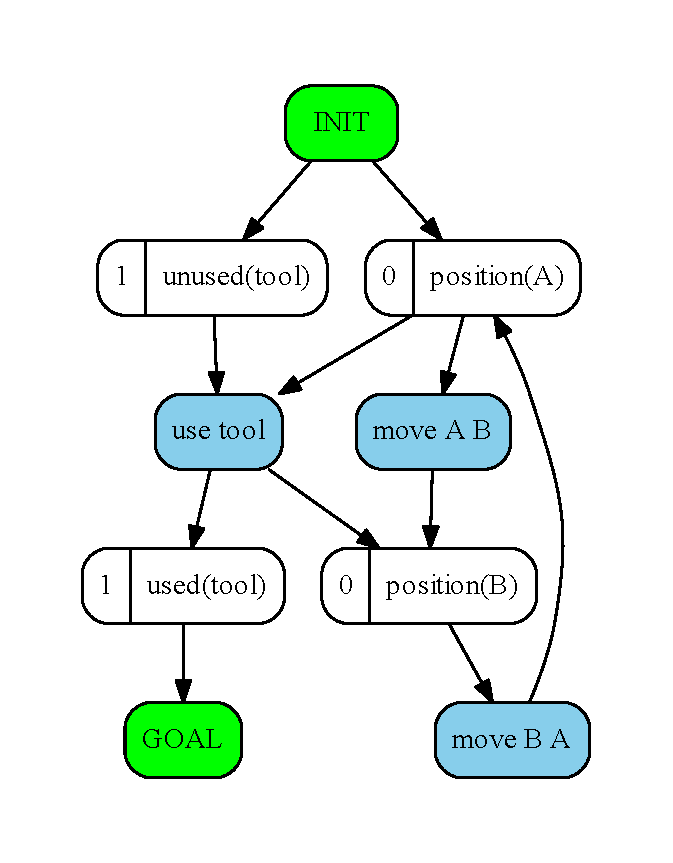
\includegraphics[scale=0.4]{mergingValues/figures/simple_input}
			\caption{before reduction}
		\end{subfigure}	
		\begin{subfigure}[b]{0.4\textwidth}
			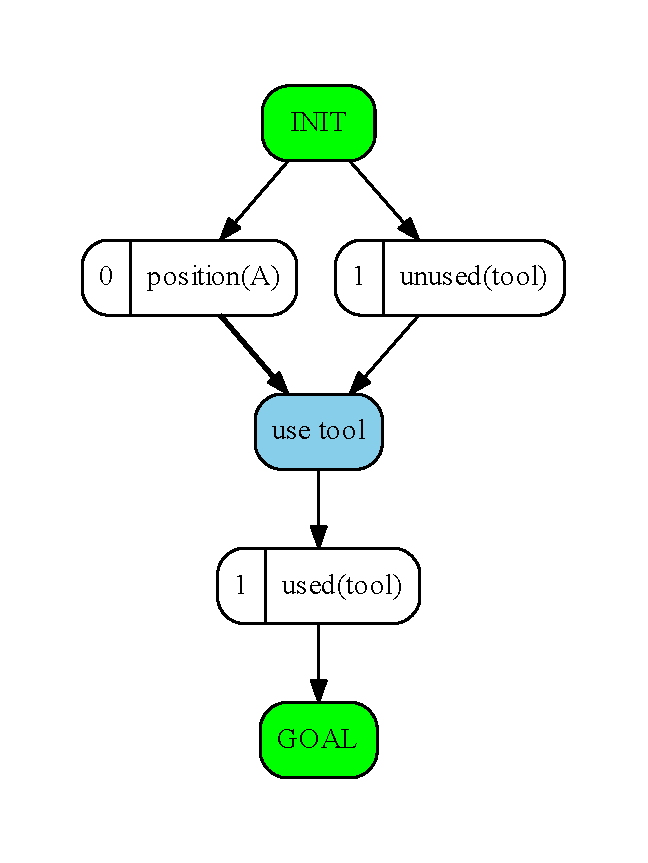
\includegraphics[scale=0.4]{mergingValues/figures/simple_output}
			\caption{after reduction}
		\end{subfigure}
		\caption{facts \emph{0 position(A)} and \emph{0 position(B)} can be merged because there are actions \emph{move A B} and \emph{move B A} switching from one fact to another without any other side effects nor preconditions}
	\end{figure}
	
	
	\section{Reduce operation}
	
	Let suppose that we have SAS in form of $<\vars, \init, \goal, \actions, \mutexes{}>$ and two actions $a_i, a_j \in \actions, a_i \neq a_j$. Operation of merging values will be done only if \ref{MSC:in:first}, \ref{MSC:in:second}, \ref{MSC:in:fourth:commonVariable} are satisfied and one of \ref{MSC:in:third:common}, \ref{MSC:in:third:2any}, \ref{MSC:in:third:1any} is satisfied.
	
	
	\begin{enumerate}
		\item $\pre{a_i} = \emptyset \land \pre{a_j} = \emptyset $ \label{MSC:in:first}
		\item $|\add{a_i}| = 1 \land |\add{a_j}| = 1 $ \label{MSC:in:second}
		\item let set $e_i \in \eff{a_i}$, $e_j \in \eff{a_j}$ and $v = \var{\add{e_i}}$
		\item $\var{\add{e_i}} = \var{\add{e_j}}$ \label{MSC:in:fourth:commonVariable}
		\item	\begin{enumerate}
			\item $\add{e_i} = \del{e_j} \land \add{e_j} = \del{e_i}$ \label{MSC:in:third:common}
			\item $\isAnyValue{\del{e_i}} \land \isAnyValue{\del{e_j}} $ \label{MSC:in:third:2any}
			\item $\isAnyValue{\del{e_i}} \land \add{e_i} = \del{e_j}$ \label{MSC:in:third:1any}
		\end{enumerate}
	\end{enumerate}
	
	Let set $u_i = \add{e_i}$ and $u_j = \add{e_j}$. This operation does following things: renames $u_j$ to $u_i$ in all occurrences in actions, mutexes, init and goal \ref{MSC:out:rename}. Then removing $u_j$ from the domain \ref{MSC:out:mergeValues}. Then effects of type $<u_i, u_i>$ are removed from operators \ref{MSC:out:changeOperators:3}. To each action, from which $<u_i, u_i>$ was removed, precondition $u_i$ is added \ref{MSC:out:addPre}. Then actions having zero effects are removed \ref{MSC:out:removeOperators}.
	
	Note that \ref{MSC:out:addPre} was added to the reduction after a bug appeared on some airport domain which was already reduced by generalize actions reduction. Adding such precondition ensures that extension operation will produce valid plan.
	
	\begin{enumerate}
		\item rename all occurrences in SAS of $u_j$ to $u_i$ \label{MSC:out:rename} \begin{enumerate}
			\item if $u_j \in \init$ then $\init{}' \leftarrow (\init \setminus \{u_j\}) \cup \{u_i\}$; else $\init{}' \leftarrow \init$
			\item if $u_j \in \goal$ then $\goal{}' \leftarrow (\goal \setminus \{u_j\}) \cup \{u_i\}$; else $\goal{}' \leftarrow \goal$
			\item $u_j$ is replaced by $u_i$ in all occurrences in $\pre{a}, \add{a}, \del{a} \forall a \in \actions$; store these actions to $\actions$
			\item $u_j$ is replaced by $u_i$ in each mutex where $u_j$ occurs; store final mutexes to $\mutexes{}'$
		\end{enumerate}	
		\item $\dom{v} := \dom{v} \setminus \{u_j\}$ \label{MSC:out:mergeValues}
		\item \begin{enumerate} 
			\item $A_c := \{a | a \in \actions, u_i \in (\del{\eff{a}} \cup \add{\eff{a}}) \}$ \label{MSC:out:changeOperators:1}
			\item remove all occurrences of effect of type $<u_i, u_i>$ in $A_c$ and store it to $A_d$ \label{MSC:out:changeOperators:2}
			\item $A_p \leftarrow \{<\pre{a} \cup \{u_i\},\eff{a}> | a \in A_d \}$ \label{MSC:out:addPre}
			\item set $A_d' := (\actions \setminus A_c) \cup A_p$ \label{MSC:out:changeOperators:3}
		\end{enumerate} 
		\item $\actions{}' := \{a | a \in A_d', \eff{a} \neq \emptyset \}$ \label{MSC:out:removeOperators}
	\end{enumerate}
	
	Afterwards, output SAS looks like $<\vars, \init{}', \goal{}', \actions{}', \mutexes{}'>$.
	
	Since we defined mutex as a set of values, so in case that $u_j$ is renamed to $u_i$ and both of them are in the same mutex, only $u_i$ remains in the mutex.
	
	
	\section{Possible outgoing states of SAS}
	
	Following states of SAS can appear after the reduction:
	
	\begin{itemize}
		\item $v$ has only one value in its domain (which can be removed by delete variable operation)
		\item mutex $m$ containing both $u_i$ and $u_j$ before the reduction, will contain only $u_i$ afterwards
		\item mutex $m$ containing $u_j$ but not $u_i$ before the reduction, will contain $u_i$ afterwards
% blbost, neni akce ktera by mela takovyhle efekty protoze by byla nesplnitelna
%		\item also note that actions has a set of effect, therefore if in step \ref{MSC:out:changeOperators:2} situation raises that $a_1$ has got effects $\{<u_n,u_j>, <u_n,u_i>\}$ and merging $u_i$ and $u_j$ is processed, after that effects of $a_1$ looks like $<u_n,u_i>$
		\item variable $v$ has at least one value
		\item after this operation a new situation in which -mv can be used may rise
	\end{itemize}
	
	
	\section{States before application of this operation}
	\begin{itemize}
		\item the original SAS
		\item after deleting variable 
		\item after another MV
	\end{itemize}
	
	
	
	\section{Reverse operation}
	
	While making this reduction, we remember $a_i$ and $a_j$. The reverse operation is done in following way:
	
	Firstly, $\dom{v} := \dom{v} \cup \{u_j\}$ and $u_i$ is renamed to $u_j$ at places (mutex, init, goal, effects, preconditions, etc) where $u_j$ was used before the merge operation.
	
	Secondly, removed operators from step \ref{MSC:out:changeOperators:3} are added and also the removed effect are added. Prevail preconditions that were added during reduction are removed.
	
	Then, to $s$ value of initial value of variable $v$ is loaded. The produced plan is then traversed, action by action. If traversed action $a$ has got $v$ in its precondition (either prevail or precondition of unconditional effect), following procedure is applied:
	
	In the case that $a$ needs $u_j$ and value $u_i$ is in $s$ then action $a_j$ is added to plan before $a$. Similar case is when $u_i$ and $u_j$ are switched, then $a_i$ is added to plan before $a$.
	
	In the case that $a$ needs $u_j$ and value $u_j$ is in $s$ then nothing is done; similar when this situation raises with value $u_i$.
	
	After each application of an action $a$ from the plan that effects variable $v$, value of $s$ is updated.
	
	Finally, after processing all actions of the plan, value in $s$ is compared with value of variable $v$ in $\goal$ and the plan is expanded by the previous method if it needs to be. The extended plan is returned as output of the reverse action.
	
	
	\section{Implementation notes}
	In implementation, while merging $u_j$ and $u_i$, value with bigger id is selected to be replaced by the other.
	
	Also, FD crashes when having a variable with only one value, therefore operation of deleting variables has to be run before running FD.
	
	